\chapter{绪论} 
\section{研究背景与相关工作}
\subsection{非线性偏微分方程精确解的研究背景与相关工作}
\subsection{非线性差分方程精确解的研究背景与相关工作}
\section{本文的选题和主要工作}
本文的主要工作分为非线性微分方程求解\zdh 非线性差分方程求解和非线性积分化简三个部分.

在非线性微分方程求解的部分, 本文首先以\Painleve{} 分析和简单Hirota方法为基础, 实现了非线性演化方程三种波解的求解. 其中, 孤子解通过简单Hirota方法获得. 获得孤子解之后, 可以通过共轭参数法得到呼吸子解, 通过长极限法得到LUMP解. 同时, 考虑到直接代数方法在微分方程求解中也存在的广泛的应用, 本文针对大规模代数方程组求解困难的问题, 设计了一个分组并行求解的算法, 并将其实现为PGSolve软件包. 作为PGSolve的应用实例, 本文实现了能够求非线性演化方程双曲正切函数解的软件包NCTM (N-order expansion method Completed Tanh Method). 本文所实现的双曲正切方法相比于已有的算法主要进行了如下改进: (1) 能够求解n+1维的方程; (2) 用n阶展开方法代替齐次平衡原则, 更加全面地考虑了方程的平衡情况.

受到在微分方程求解中被广泛应用的齐次平衡原则的启发, 本文将其用于求解非线性差分方程的多项式解. 齐次平衡原则通过平衡方程中两个不同的最高次项的次数来确定解的次数, 只能在一些情况下生效. 本文考虑同时平衡方程中最高$n$项的次数和系数, 提出了$n$阶展开方法来处理齐次平衡原则不能处理的情况. 同时, 本文将$n$阶展开方法实现为一个便于拓展应用的Maple软件包NEM (N-order Expansion Method). 基于NEM, 我们实现了能够求解非线性差分方程所有多项式解的软件包NLREPS (Non-Linear Recurrence Equation Polynomial Solution Solver). 同时其它需要用到齐次平衡原则的方法也能迅速地用NEM进行完善. 例如NTCM就是用NEM替代齐次平衡方法进行完善的. 同时, \Painleve{} 分析的过程中也用到了齐次平衡原则, 因此我们也以\Painleve{} 分析为例展示了如何用NEM替代齐次平衡原则.

因为在非线性微分方程求解的过程中往往需要进行非线性积分表达式化简. 因此, 我们也将非线性积分化简作为一个具有挑战性的任务进行探索. 在这个部分, 本文基于导数的乘法规则, 设计了一个递归算法来寻找积分表达式中的所有二项合并规则. 然后, 基于这些规则, 本文设计了一个线性规划模型用于求解输入表达式的最简形式.

\begin{figure}[htbp]
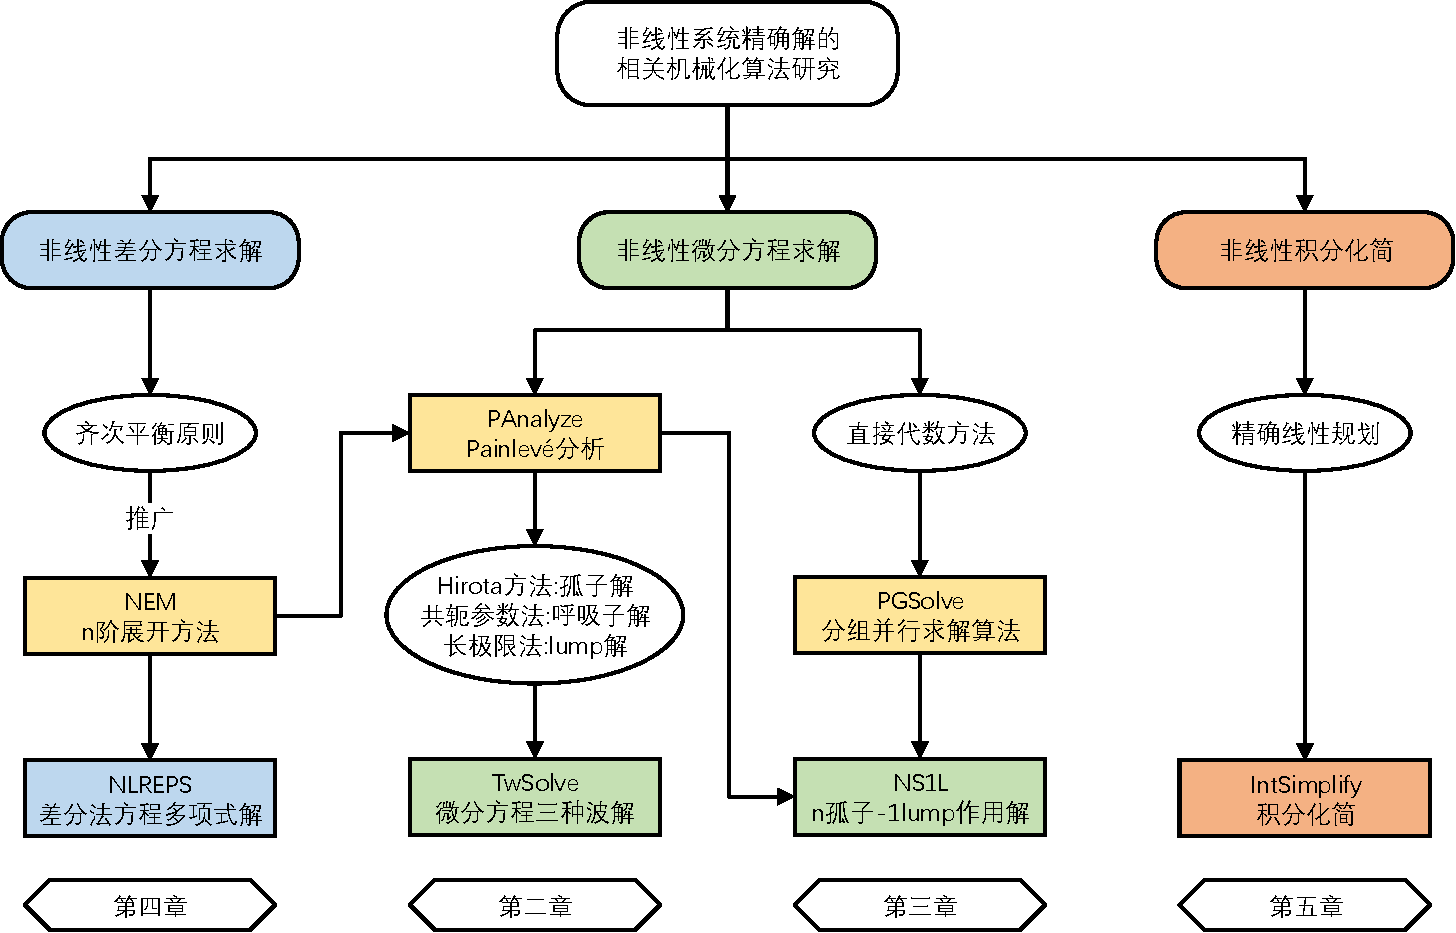
\includegraphics[width=\textwidth]{fig/outline.pdf}
\caption{本文工作大纲图}\label{outline}
\end{figure}

综上所述, 本文主要工作可以总结为如\reffig{outline}所示的框架. 在\reffig{outline}中, 椭圆表示方法\zdh 矩形表示软件包. 其中, 软件包元素的第一行是软件包的名称, 第二行是软件包用途的简要说明. 软件包以4种颜色进行区分, 黄色表示基础工具, 蓝色表示用于求解差分方程, 绿色表示用于求解微分方程, 粉色表示用于进行积分化简. 即, 对于微分\zdh 差分\zdh 积分这三种不同的非线性系统的一些具体问题, 本文共设计了7个算法, 并实现了7个Maple软件包.
